\begin{exercise}
In Example 4.1, if $\pi$ is the equiprobable random policy, what is $q_\pi(11, \mathit{down})$?

\begin{figure}[H]
    \centering
    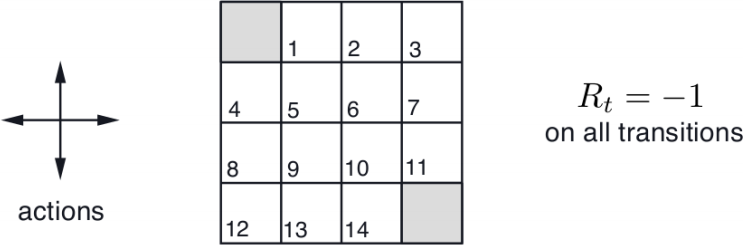
\includegraphics[width = 0.5 \textwidth]{3.22.png}
    \caption{Example 4.1}
    \label{fig:3.22.1}
\end{figure}

\end{exercise}

\begin{solution}
  After taking action $down$ in state $11$ we get a reward of $-1$ and land in a terminal state, so

  \begin{align*}
    q_\pi(11, down)
    =
    \mathbb{E}_\pi\big[G_t \mid S_t = 11, A_t = down\big]
    =
    \mathbb{E}_\pi\big[R_{t+1} \mid S_t = 11, A_t = down\big]
    =
    -1
  \end{align*}
\end{solution}
